\documentclass{beamer}
\usetheme{metropolis}
\usepackage{graphicx}
\usepackage{subfig}
\title{Calculus-Based Physics-1: Mechanics (PHYS150-01): Week 3}
\date{September 18th - September 22nd, 2017}
\author{Jordan Hanson}
\institute{Whittier College Department of Physics and Astronomy}

\begin{document}
\maketitle

\section{Week 2 Review}

\begin{frame}{Week 2 Review}
\begin{enumerate}
\item Displacement, and instantaneous velocity and acceleration
\begin{itemize}
\item \textit{Mathematics review}: taking derivatives
\item Average velocity and average acceleration
\end{itemize}
\item The case of constant acceleration
\begin{itemize}
\item An \textit{an equation of motion} for constant acceleration
\item Derivation of \alert{common equations of motion}
\item Average quantities and exercises
\end{itemize}
\item \textbf{Lab Activity: Measuring acceleration of gravity: \textit{g}}
\item Exercises with vectors, graphs, and equations of motion
\end{enumerate}
\end{frame}

\section{Week 2 Review Problems}

\begin{frame}{Week 2 Review Problems}
\small
\begin{minipage}[b]{0.45\linewidth}
If a subway train is moving to the left (has a negative velocity) and then comes to a stop, what is the direction of its acceleration? Is the acceleration positive or negative?
\begin{itemize}
\vspace{0.5cm}
\item A: To the right, positive
\item B: To the right, negative
\item C: To the left, positive
\item D: To the left, negative
\end{itemize}
\end{minipage}
\hspace{0.5cm}
\begin{minipage}[b]{0.45\linewidth}
An object that is thrown straight up falls back to Earth.  When is its velocity zero?  Does its velocity change direction?  Does the acceleration change sign?
\begin{itemize}
\item A: During flight, yes, no
\item B: At the peak height, yes, yes
\item C: At the peak height, yes, no
\item D: During flight, no, no
\end{itemize}
\end{minipage}
\end{frame}

\section{Week 3 Summary}

\begin{frame}{Week 3 Summary}
\begin{enumerate}
\item Displacement, velocity and acceleration vectors \alert{as functions of time}
\begin{itemize}
\item Breaking into components
\item Derivatives of components
\end{itemize}
\item Combining free-fall and vector components: \alert{projectile motion}
\begin{itemize}
\item The independence of velocity components
\item \textbf{Lab-activity: testing component independence}
\end{itemize}
\item Relative motion and reference frames
\begin{itemize}
\item Relative motion in one-dimension
\item Relative motion in two-dimensions
\end{itemize}
\end{enumerate}
\end{frame}

\section{Vectors as functions of time}

\begin{frame}{Vectors as functions of time}
In general, the displacement of an object depends on time:
\begin{equation}
\vec{r}(t) = x(t) \hat{i} + y(t) \hat{j} + z(t) \hat{k}
\end{equation}
\begin{itemize}
\item $x(t)$ is the displacement in the x-direction
\item $y(t)$ is the displacement in the y-direction
\item $z(t)$ is the displacement in the z-direction
\end{itemize}
\end{frame}

\begin{frame}{Vectors as functions of time}
\begin{figure}
\centering
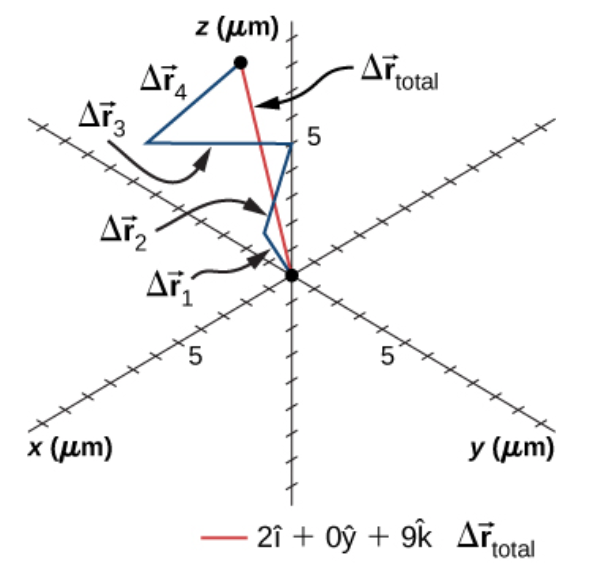
\includegraphics[width=0.6\textwidth,trim=0cm 2cm 0cm 0cm,clip=true]{figures/Brownian.png}
\caption{\label{fig:brown} An example of a displacement vector at different moments in time.}
\end{figure}
\end{frame}

\begin{frame}{Vectors as functions of time}
The particle in Fig. \ref{fig:brown} has four displacement vectors at four moments in time:
\begin{itemize}
\item $\vec{r}_{\rm 1} = 2.0\hat{i} + 1.0\hat{j} + 3.0\hat{k}\quad(\mu m)$ at $t_{\rm 1}$
\item $\vec{r}_{\rm 2} = -1.0\hat{i} + 0.0\hat{j} + 3.0\hat{k}\quad(\mu m)$ at $t_{\rm 2}$
\item $\vec{r}_{\rm 3} = 4.0\hat{i} + -2.0\hat{j} + 1.0\hat{k}\quad(\mu m)$ at $t_{\rm 3}$
\item $\vec{r}_{\rm 4} = -3.0\hat{i} + 1.0\hat{j} + 2.0\hat{k}\quad(\mu m)$ at $t_{\rm 4}$
\end{itemize}
What is the total displacement of the particle from the origin?
\end{frame}

\begin{frame}{Vectors as functions of time}
We can think of this type of problem as an accounting problem, lining up columns (units: $\mu m$):
\begin{figure}
\begin{tabular}{| c | c | c | c | c |}
\hline
$t_{\rm i}$ & $\vec{r}_{\rm i}(t_{\rm i})$ & $x(t_{\rm i})$ & $y(t_{\rm i})$ & $y(t_{\rm i})$ \\
\hline
$t_{\rm 1}$ & $\vec{r}_{\rm 1}(t_{\rm 1})$ & 2.0 & 1.0 & 3.0 \\
\hline
$t_{\rm 2}$ & $\vec{r}_{\rm 2}(t_{\rm 2})$ & -1.0 & 0.0 & 3.0 \\
\hline
$t_{\rm 3}$ & $\vec{r}_{\rm 3}(t_{\rm 3})$ & 4.0 & -2.0 & 1.0 \\
\hline
$t_{\rm 4}$ & $\vec{r}_{\rm 4}(t_{\rm 4})$ & -3.0 & 1.0 & 2.0 \\
\hline
\hline
$t_{\rm total}$ & $\vec{r}_{\rm total}(t_{\rm total})$ & 2.0 & 0.0 & 9.0 \\
\hline
\end{tabular}
\caption{\label{tab:account} Accounting for the different displacement components, in units of $\mu m$.}
\end{figure}
\end{frame}

\begin{frame}{Vectors as functions of time}
\begin{figure}
\centering
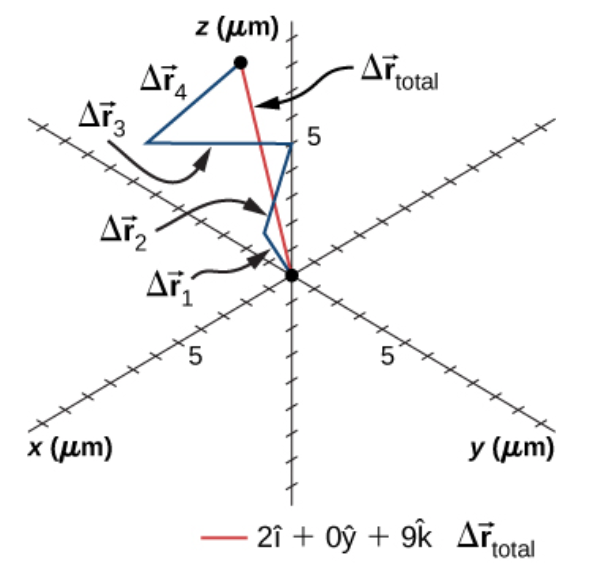
\includegraphics[width=0.6\textwidth]{figures/Brownian.png}
\caption{\label{fig:brown2} The total displacement of the particle is $\vec{r}_{\rm total} = 2.0\hat{i} + 0.0\hat{k} + 9.0\hat{k}\quad (\mu m)$.}
\end{figure}
\end{frame}

\begin{frame}{Vectors as functions of time}
\small
The 18th hole at Pebble Beach Golf Course is a dogleg to the left of length 496.0 meters.  The fairway off the tee is taken to be the x direction.  A golfer hits his tee shot a distance of 300 meters, corresponding to a displacement of $\vec{r}_{\rm 1} = 300.0 \hat{i} \quad (m)$, and then hits a second shot 189.0 meters with $\vec{r}_{\rm 2} = 172.0 \hat{i} + 80.3 \hat{j} \quad m$.  What is the final displacement from the tee?
\begin{itemize}
\item A: $\vec{r}_{\rm final} = 172.0 \hat{i} + 80.3\hat{j}\quad (m)$
\item B: $\vec{r}_{\rm final} = 172.0 \hat{i} + 380.3\hat{j}\quad (m)$
\item C: $\vec{r}_{\rm final} = 472.0 \hat{i} + 0.0\hat{j}\quad (m)$
\item D: $\vec{r}_{\rm final} = 472.0 \hat{i} + 80.3\hat{j}\quad (m)$
\end{itemize}
\end{frame}

\begin{frame}{Vectors as functions of time}
\small
If the first shot takes 5.0 seconds, the second shot takes 4.0 seconds, and the walking time in between the shots is 60.0 seconds, what is the average velocity vector for the ball after the two shots?
\begin{itemize}
\item A: $\vec{r}_{\rm final} = 1.7 \hat{i} + 8.3\hat{j}\quad (m/s)$
\item B: $\vec{v}_{\rm final} = 172.0 \hat{i} + 80.3\hat{j}\quad (m/s)$
\item C: $\vec{v}_{\rm final} = 6.8 \hat{i} + 1.2\hat{j}\quad (m)$
\item D: $\vec{v}_{\rm final} = 6.8 \hat{i} + 1.2\hat{j}\quad (m/s)$
\end{itemize}
\end{frame}

\begin{frame}{Vectors as functions of time}
The prior problem indicates something you may already have guessed:
\begin{equation}
\vec{v}_{\rm avg}(t) = v_{\rm x}(t) \hat{i} + v_{\rm y}(t) \hat{j} + v_{\rm z}(t) \hat{k} = \frac{\Delta\vec{r}}{\Delta t}
\label{eq:vel}
\end{equation}
\begin{itemize}
\item $v_{\rm x}(t)$ is the avg. velocity in the x-direction
\item $v_{\rm y}(t)$ is the avg. velocity in the y-direction
\item $v_{\rm z}(t)$ is the avg. velocity in the z-direction
\end{itemize}
In other words, we divide each displacement component by the time, to get a vector where each component is the average velocity in that direction.  $\Delta\vec{r} = \vec{r}_{\rm f} - \vec{r}_{\rm i}$.
\end{frame}

\begin{frame}{Vectors as functions of time}
Instantaneously, Eq. \ref{eq:vel} is true, if we \alert{take the limit} $\Delta t \to 0$:
\begin{equation}
\vec{v}(t) = \lim_{\Delta t \to 0} \frac{\Delta\vec{r}}{\Delta t} = \frac{dx}{dt}\hat{i} + \frac{dy}{dt}\hat{j} + \frac{dz}{dt}\hat{k}
\label{eq:vel2}
\end{equation}
\begin{itemize}
\item $\frac{dx}{dt}$ is the instantaneous velocity in the x-direction
\item $\frac{dy}{dt}$ is the instantaneous velocity in the y-direction
\item $\frac{dz}{dt}$ is the instantaneous velocity in the z-direction
\end{itemize}
\end{frame}

\begin{frame}{Vectors as functions of time}
The position of a particle is $\vec{r}(t) = 4.0t^2\hat{i} - 3.0 \hat{j} + 2.0t^2\hat{k}$ (m).  What is the velocity vector at $t=2$ seconds?  What is the average velocity between $t=0$ and $t=2$ seconds?
\begin{itemize}
\item A: $16\hat{x} + 8\hat{z}$ (m/s), $8\hat{x} + 4\hat{z}$ (m/s)
\item B: $8\hat{x} + 4\hat{z}$ (m/s), $4\hat{x} + 2\hat{z}$ (m/s)
\item C: $8\hat{x} + 8\hat{z}$ (m/s), $4\hat{x} + 4\hat{z}$ (m/s)
\item D: $4\hat{x} + 2\hat{z}$ (m/s), $4\hat{x} + 2\hat{z}$ (m/s)
\end{itemize}
\end{frame}

\begin{frame}{Vectors as functions of time}
Instantaneously, from Eq. \ref{eq:vel2}: 
\begin{equation}
\vec{a}(t) = \lim_{\Delta t \to 0} \frac{\Delta\vec{v}}{\Delta t} = \frac{dv_{\rm x}}{dt}\hat{i} + \frac{dv_{\rm y}}{dt}\hat{j} + \frac{dv_{\rm z}}{dt}\hat{k}
\label{eq:vel3}
\end{equation}
\begin{itemize}
\item $\frac{dv_{\rm x}}{dt}$ is the instantaneous acceleration in the x-direction
\item $\frac{dv_{\rm y}}{dt}$ is the instantaneous acceleration in the y-direction
\item $\frac{dv_{\rm z}}{dt}$ is the instantaneous acceleration in the z-direction
\end{itemize}
\end{frame}

\begin{frame}{Vectors as functions of time}
The velocity of a particle is $\vec{v}(t) = 8.0t\hat{i} + 4.0t\hat{k}$ (m/s).  What is the acceleration vector at $t=2$ seconds?  What is the average acceleration between $t=0$ and $t=2$ seconds?
\begin{itemize}
\item A: $4\hat{i} + 4\hat{k}$ (m/s$^2$), $2\hat{i} + 2\hat{k}$ (m/s$^2$)
\item B: $8\hat{i} + 4\hat{k}$ (m/s$^2$), $8\hat{i} + 4\hat{k}$ (m/s$^2$)
\item C: $8\hat{i} + 8\hat{k}$ (m/s$^2$), $4\hat{i} + 4\hat{k}$ (m/s$^2$)
\item D: $4\hat{i} + 8\hat{k}$ (m/s$^2$), $2\hat{i} + 4\hat{k}$ (m/s$^2$)
\end{itemize}
\end{frame}

\begin{frame}{Vectors as functions of time}
\small
The displacement of a particle is $\vec{x}(t) = (2t+3)\hat{i}+(\frac{3}{2}t^2+2t+3.0)\hat{j}$ (m).  What is the horizontal velocity (the $\hat{i}$-component of the velocity) at $t=4$ seconds?  At $t=10$ seconds?
\begin{itemize}
\item A: 4 m/s, 4 m/s
\item B: 2 m/s, 4 m/s
\item C: 2 m/s, 2 m/s
\item D: 4 m/s, 2 m/s
\end{itemize}
\end{frame}

\begin{frame}{Vectors as functions of time}
\small
The displacement of a particle is $\vec{x}(t) = (2t+3)\hat{i}+(\frac{3}{2}t^2+2t+3.0)\hat{j}$ (m).  What is the vertical velocity (the $\hat{j}$-component of the velocity) at $t=4$ seconds?  At $t=10$ seconds?
\begin{itemize}
\item A: 14 m/s, 32 m/s
\item B: 32 m/s, 14 m/s
\item C: 12 m/s, 30 m/s
\item D: 30 m/s, 12 m/s
\end{itemize}
\end{frame}

\begin{frame}{Vectors as functions of time}
Notice in the previous example, the x-velocity and y-velocity were not the same function. \\
\vspace{0.5cm}
In the kinematic description of motion, \alert{\textit{we are able to treat the different components of motion separately.}}  In many cases, motion in the horizontal direction does not affect motion in the vertical direction, and vice versa.\\
\vspace{0.5cm}
\small
\framebox[1.1\width]{\textbf{Motions in displacement components are independent.}} \\
\vspace{1cm}
\textit{(Exception: non-conservative forces.  More on this later.)}
\end{frame}

\section{Combining free-fall and vector components: projectile motion}

\begin{frame}{Projectile motion}
\small
\begin{figure}
\centering
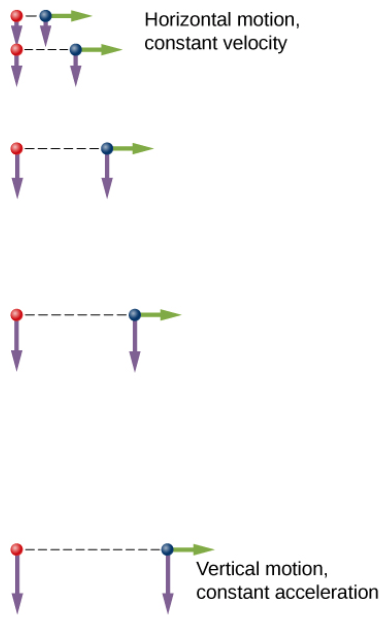
\includegraphics[width=0.35\textwidth]{figures/fall.png}
\caption{\label{fig:fall} The red particle accelerates vertically, with no horizontal velocity.  The blue particle acclerates vertically, with some horizontal velocity.}
\end{figure}
\end{frame}

\section{Lab Activity}

\begin{frame}{Projectile motion}
Is this true?  Figure \ref{fig:fall} is testable by experiment. \\
\vspace{0.5cm}
\small
Procedure:
\begin{enumerate}
\item Obtain two marbles, a meter stick, and a stopwatch.
\item Measure the height of the lab bench, $\Delta x$.
\item We are going to drop a marble from this height ($\Delta x$) and record the time.  Show first algebraically that the predicted time for the marble to fall is $t = \sqrt{2\Delta x/g}$.
\item Measure $t$ for several trials.  Does it match the expected result $\sqrt{2\Delta x/g}$?  What are sources of error?
\item Repeat the measurement, but \textbf{roll the marble off of the table instead of dropping it} from $\Delta x$.  Does the average result for $t$ change?
\end{enumerate}
\end{frame}

\section{Answers}

\begin{frame}{Answers}
\begin{columns}[T]
\begin{column}{0.5\textwidth}
\begin{itemize}
\item To the right, positive
\item At the peak height, yes, yes
\item $\vec{r}_{\rm final} = 472.0 \hat{i} + 80.3\hat{j}\quad (m)$
\item $\vec{v}_{\rm final} = 6.8 \hat{i} + 1.2\hat{j}\quad (m/s)$
\item $16 \hat{x} + 8\hat{z}$ (m/s), $8\hat{x} + 4\hat{z}$ (m/s)
\item $8\hat{i} + 4\hat{k}$ (m/s$^2$), $8\hat{i} + 4\hat{k}$ (m/s$^2$)
\item 2 m/s, 2 m/s
\item 14 m/s, 32 m/s
\end{itemize}
\end{column}
\begin{column}{0.5\textwidth}
\begin{itemize}
\item 
\end{itemize}
\end{column}
\end{columns}
\end{frame}

\end{document}
